% !TeX encoding=utf8
% !TeX spellcheck = de-CH

\chapter{Analyse}

\section{Allgemein}
Wieso braucht es Zeitsynchronisation? Was für Probleme und Schwierigkeiten können dabei auftreten? Diese Fragen aus der Aufgabenstellung werden in den nachfolgenden Kapiteln detailliert beantwortet.

\subsection{Hintergründe}
In der heutigen Zeit sind wir es uns gewohnt, dass wir uns darauf verlassen können das unsere Uhren in der Regel die gleiche Zeit anzeigen. 
Wie war das früher? Heute würde vieles nicht mehr funktionieren, wenn wir keine Uhren hätten, bzw. die Uhren nicht synchronisiert werden, oder etwa doch?

\subsubsection{Kurzer Rückblick in die Geschichte}
%http://www.astro-siggi.de/tutorial-funkuhr.html
%http://de.wikipedia.org/wiki/Geschichtliche_Entwicklung_der_Zeit%C3%BCbertragung_per_Funk
%http://en.wikipedia.org/wiki/Time_signal
\subsubsection{Was wäre wenn...}
%Stichwort: GPS, Börse, ÖV, 

\subsection{Was für Schwierigkeiten können dabei auftreten?}
%http://diepresse.com/home/spectrum/zeichenderzeit/695559/Auf-der-Hohe-der-Zeit

\subsection{Atomuhr}
%http://www.meinberg.de/german/info/atomic_clock.htm
Defition:
\begin{quote}
Eine Atomuhr ist ein Zeitmesser, dessen Zeitnormal die hochfrequente Schwingungsdauer bestimmter Atome ist (z.B. Caesium, Rubidium), die durch ein elektromagnetisches Feld oder optisches Pumpen zu Schwingungen angeregt werden und einen Quarzgenerator synchronisieren.
\end{quote} % http://www.meinberg.de/german/info/atomic_clock.htm
Die Atomuhr wurde vom Amerkikaner Isidor Isaac Rabi (1898-1988) erfunden. 1944 wurde der Erfinder mit dem Nobelpreis belohnt.
%Quelle http://www.meinberg.de/german/info/atomic_clock.htm

\subsection{Funkuhr}
Im Gegensatz zur Atomuhr, kann eine Funkuhr nicht selbst die korrekte Zeit berechnen. Sie hat einen Funkempfänger eingebaut, der von einen "`echten"' Atomuhr das Funksignal empfangen kann und darus die genaue Uhrzeit annäheren kann. Der erstmalige Zeitabgleich dauert je nach Synchronisationstyp wenige Minuten. Sobald der Decode Prozess abeschlosse ist, läuft die Uhr synchronisiert.

Die Genauigkeit einer Funkuhr liegt im Schnitt zwischen 5 und 25 msec.

%Quartzuhren...
%http://de.wikipedia.org/wiki/Funkuhr
%http://www.heret.de/funkuhr/index.htm

\section{Möglichkeiten der Zeitsynchronisation}
Grundsätzlich stehen mit dem heutigen Stand der Technik die nachfolgend im Detail beschriebenen Möglichkeiten zur Zeitsynchronisation zur Verfügung.

\subsection{Funk}
Funk, bwz. Funkwellen sind allgegenwärtig und aus dem heutigen Alltag nicht mehr Weg zu denken.

\subsection{Zeitsignaldienste}
Zeitsignal Dienste sind untereinander mit höchster Genaugigkeit und Präzision vernetzt. Die von diesen Diensten ermittelte Zeit stimmt in weiten Bereichen weit unter Nanosekunden überein.(Weltzeit: UTC). Koordination durch Erdrotations-Dienst (IERS)

\subsection{Zeitzeichensender - Allgemein}
Zeitzeichensender senden in bestimmten Zeitabständen codierte Zeitinformationen. Funkuhren und entsprechende Geräte können diese Signale empfangen, decodieren und interpretieren. Die Zeit und das Datum auf dem Gerät wird dann mit denen des Signales abgeglichen. Um eine erfolgreiche Synchronisierung zu erreichen muss dass Signal eine gewisse Zeit empfangen werden. Vielfach dient für das Signal mit den Zeitinformationen eine Normalfrequenz als Grundlage.

Die Zeitzeichensender benötigen nicht zwingend eine spezielle Sendeanlage, vielfach werden die Signale über einen Rundfunksender übermittelt.

Die Signal werden in der Regel im Sekundentakt übermittelt (Ausnahme: Russische Sender senden zum Beispiel zum Teil im Zehntelsekundentakt). Damit ein Minutenwechsel einfach und eindeutig identifiziert werden kann wird bei der Sekunde 0 / 59 eine Minutenkennung gesendet.

Die Codierung der Sender ist nicht vereinheitlicht, hat jedoch mehrheitlich eine ähnliche Struktur und basiert auf einer 60-Bit (bzw. 59) Codierung. Die Codierung und das Signal sind so ausgelegt, dass diese einfach von Maschinen verarbeitet und interpretiert werden können.

Das Signal wird am Sendestandort an in der unmittelbaren Nähe in der Regel von mehreren Atomuhren generiert und miteinander abgeglichen. Dadurch wird eine sehr hohe Genauigkeit erreicht. Wird die Distanz und die Signallaufzeit zwischen Sender und Empfänger berücksichtigt, ist die Genauigkeit im Nanosekundenbereich angesiedelt. Pro 300 km beträgt die Verzögerung ca. 1 ms.

Das Signal wird entweder als Langwelle, Mittelwelle oder als Kurzwelle ausgesendet. An einigen Standorten wird sogar auf Langstwellen oder Ultrakurzwellen gesendet.
Jeder Zeitzeichensender verfügt über ein eindeutiges Kennzeichen...
%dUT1: Differenz Erdrotationszeit und Atomzeit	
%http://de.wikipedia.org/wiki/Zeitzeichensender

\subsubsection{Frequenznormale}
Bis in die 70er Jahre wurde oft das Signal von Radiostationen als Frequenznormale ausgewertet.
Vorstufe Zeitzeichensender, hochgenaue Schwingungsfrequenz, Empfänger muss einmal eingestellt werden, anschliessend werden Schwingungen gezählt. Radio z.B Langwellensender mit 150 kHz oder Stromnetz mit 50 oder 60 Hz

\subsubsection{Zeitzeichensender in der Schweiz}

\begin{wrapfigure}{r}{0.6\textwidth}
  \begin{center}
    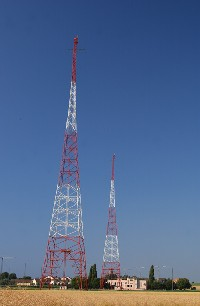
\includegraphics[width=0.6\textwidth]{./images/Analyse/Prangings_VD_CH.jpg}
  \end{center}
  \caption[Zeitzeichensender in Prangins (VD)]{Zeitzeichensender in Prangins (VD) (Quelle: Eigenössisches Institut für Metrologie (METAS); \url{http://www.metas.ch/root_legnet/Web/Fachbereiche/Zeit_Frequenz/dissemination/HBG})} 
\end{wrapfigure}

In der Schweiz war zwischen 1966 und 2011 der Zeitzeichensender HBG in Prangins (VD) in Betrieb. Aufgrund mangelnder Nachfrage wurde der Sendebetrieb Ende 2011 eingestellt und die Sendeanlage gesprengt und abgebaut. Der Sender wurde vom Eigenössischen Institut für Metrologie betrieben und sendete mit einer Frequenz von 75 kHZ.

\subsection{Zeitzeichensender - DCF77}
DCF77 bezeichnet einen Zeitzeichensender in Deutschland (Mainflingen in Mainhausen) der von der Physikalisch-Technischen Bundesanstalt in Braunschweig (PTB) entwickelt wurde. Der Betrieb erfolgt durch die Media Broadcast GmbH. Die Bezeichnung setzt sich aus D für Deutschland, C für Langwellensender, F für Frankfurt (Mainhausen liegt in der Nähe von Frankfurt) und 77 für die Sendefrequenz (77.5 kHz).

Langwellensender
%Seit 1959: Normalfrequenz (Eichfrequenz, hochgenaue Frequenz, häufig identisch mit Trägerfrequenz von Zeitzeichendiensten und Rundfunksendern im Lang- und Mittelwellenbereich)

Der DCF77 sendet im Sekundenrythmus die aktuelle mitteleuropäische Zeit, bzw. mitteleuropäische Sommerzeit. Seit 1973 werden Datum und Uhrzeit gesendet.

Früher wurde das Rufzeichen des Senders während der 20. bis 32. Sekunde der Minuten 19, 39 und 59 ausgesendet. Es wurde aber festgestellt, dass dieses Signal eine Verschlechterung des Signal-zu-Rausch-Abstandes zur Folge hatte. Das Signal des DCF77 kann auch ohne Rufzeichen eindeutig identifiziert werden.

Die ausgesendete Zeit wird mit einer am PTB entwickelten Steuereinrichtung auf Basis von drei Atomuhren ermittelt. Das daraus erhaltene Signal wird mit den primären Atomuhren des PTB synchronisiert. Aktuell sind dort zwei Caesium-Uhren und zwei Caesium-Fontänen im Einsatz. Das Endsignal hat eine Genauigkeit von $10^{-12}$. Daraus resultiert ein Fehler von ca. einer Sekunde in 30'000 Jahren.

Erzeugung des Signals durch PTB, Aussendung durch Telekom


Das Signal wird von drei Steuereinheiten unabhängig voneinander erzeugt. Stimmt das Signal der Hauptsteuereinheit nicht mit den Signalen der Reserveeinheiten überein, wird auf eine Reserveeinheit umgestellt. Sind alle drei Signal unterschiedlich, wird die Signalaussendung unterbrochen.

Das DCF77 Signal hat je nach Wetterlage, Tages- und Jahreszeit eine Reichweite von 2'000 km. Da der Zeitcode durch Amplitudenmodulation erfolgt kann das Signal leicht gestört werden, z.B. durch Gewitter. Bei Gewitter / Sturm oder starken Winden wird die Antenne vorübergehend ausser Betrieb genommen, da durch die Schwingung der Antenne eine messbare Phasenmodulation bei den Empfängern entsteht.

Der Sender sendet mit 50 kW (nominell).

Neben der Normalfrequenz wird seit 1973 zusätzlich ein Digitales Signal gesendet welches Informationen zu Datum und Uhrzeit enthält.

Im Signal ist die Zeitinformation der nächsten Minute kodiert. 
%DCF-77
%http://www.cyber-sciences.com/support/technical_dcf77.html
%http://de.wikipedia.org/wiki/DCF77
%http://www.dcf77.de/
%http://www.bmvit.gv.at/telekommunikation/publikationen/infoblaetter/downloads/042013.pdf
%Wetter
\subsubsection{Codierung}
\begin{tabular}{p{0.5cm} p{13.5cm}}
\textbf{Bit} & \textbf{Bedeutung} \\ \hline
0 & Start einer Minute \\
1-14 & Wetterinformationen und Katastrophenschutz \\ \hline
\multicolumn{2}{p{14cm}}{\textit{Informationen zu Unregelmässigkeiten im Sendebetrieb, Zeitzone, Beginn / Ende Sommerzeit, Schaltsekunden}}  \\ \hline
15 & Rufbit \\
16 & Wenn Wert 1: Umstellung MEZ/MESZ am Ende der Stunde \\
17 & Wenn Wert 0: MEZ, Wenn Wert 1: MESZ \\
18 & Wenn Wert 0: MESZ, Wenn Wert 1: MEZ \\
19 & Wenn Wert 1: Schaltsekunde am Ende der Stunde. \\ \hline
\multicolumn{2}{p{14cm}}{\textit{Zeitinformation der nachfolgenden Minute in BCD-Zahlen (Start mit LSB). Gerade Parität für Fehlererkennung. Erster Wochentag ist der Montag (Tag 1)}}  \\ \hline
20 & Beginn der Zeitinformation (immer 1) \\
21 & Minute (Einer) - Bit für 1 \\
22 & Minute (Einer) - Bit für 2 \\
23 & Minute (Einer) - Bit für 4 \\
24 & Minute (Einer) - Bit für 8 \\
25 & Minute (Zehner) - Bit für 10 \\
26 & Minute (Zehner) - Bit für 20 \\
27 & Minute (Zehner) - Bit für 40 \\
28 & Parität Minute \\ \hline
29 & Stunde (Einer) - Bit für 1 \\
30 & Stunde (Einer) - Bit für 2 \\
31 & Stunde (Einer) - Bit für 4 \\
32 & Stunde (Einer) - Bit für 8 \\
33 & Stunde (Zehner) - Bit für 10 \\
34 & Stunde (Zehner) - Bit für 20 \\
35 & Parität Stunde \\ \hline
\end{tabular}

\subsubsection{Network Time Protocol}
Wird bei eine NTP-Root-Server (Siehe Kapitel \ref{Analyse:Internet}) das DCF77-Signal als Referenz verwendet wird dieser mit der Kennung "`.DCFa"' versehen.

\subsection{GPS}
Nebst der Zeitsynchronisation über Funk, kann eine genaure Information aus den GPS-Satelliten gewonnen werden. Dies obwhol GPS-Systeme hauptsächlich zur Lokalisierung des Standortes entwickelt wurden.
Momentan befinden sich sechs solche Satelliten auf ungefähr 200'000km Höhe. Jeder umrundet die Erde zweimal pro Tag. Auf jedem Satellit sind jeweils zwei Atomuhren vorhanden.
Ein Satellit sendet dauernd seine Bahnposition und die genaue Uhrzeit. Durch Signale mehrere Satelliten, kann der Empfänger seinen genauen Standort ermitteln.
Anschliessend kann die Laufzeit des Signals zurück gerechnet werden und die durchs Versenden verstrichene Zeit, das Delay, approximiert werden.
Durch dieses Verfahren kann die Uhrzeit, mit einer Genauigkeit unter 1${\mu}sec$, berechnet werden.

Vorteile der Zeit-Synchronisation über GPS sind: weltweilte Abdeckung und hohe sehr hohe Genauigkeit.

Ein grosser Nachteile der GPS Synchronisation ergibt sich jedoch durch das verwendete Kurzwellen Signal (zwischen 1176,45 bis 1575,42 MHz). Dieses Signal kann nur unter freien Himmel empfangen werden und eignet sich daher nicht für einen typischen Computer.

%GPS: http://www.mono.rgbtechnology.pl/de/faq/gps-zeitsynchronisation.html
%http://www.stardado.de/1244, http://www.emsec.rub.de/media/crypto/attachments/files/2010/04/ms_michael_ziaja.pdf
%GPS vs DCF77: http://www.hopf.com/de/dcf77-gps_de.html
\subsection{Internet} \label{Anaylse:Internet}

Will man eine Uhr via Internet synchronisieren, stösst man rasch auf folgendes Problem:

\begin{verse}
Die genaue Senddauer eines  Datenpaktes, welches die der korreketen Uhrzeit beinhaltet, ist weder vorhersehbar noch kan man die verstrichene Zeit beim Empfänger zurückrechnen.
\end{verse}

Da keine Aussagen über die Genauigkeit der empfangenen Information möglich ist, verliert sie drastisch an Wert.

\section{Zeitprotokoll}
Um eine brauchbare Synchronisation via Internet zu ermöglichen wurde folgender, vereinfachter Datenaustausch definiert: (Der Client synchronisiert seine Zeit mit der genauen Zeit eines Server. Die Serverzeit entspricht also nicht der Clientzeit.)\cite{ntp_stackoverfow}

\begin{enumerate}
\item Der Client schickt eine \textbf{Anfrage an den Server} und \textbf{merkt} sich seine aktuelle, lokale Zeit (welche mit grosser Wahrscheinlichkit nicht der korrekten Serverzeit entspricht).
\item Der Server antwortet mit seiner lokalen, korrekten \textbf{Zeit des Empfangs und der des Rückversandes}.
\item Der Client merkt sich die Zeit des Empfangs der Antwort. 
\end{enumerate}
\vspace{1em}
Nach dem Datenaustausch hat der Client folgende vier verschiedene Zeiten zur Verfügung:
\begin{enumerate}
\item Client: lokale Zeit bei der Anfrage - (A)
\item Server: Empfangszeit - (X)
\item Server: Versandzeit - (Y)
\item Client: Empfangszeit - (B)
\end{enumerate}
\vspace{1em}
Als Annahme wird vereinfacht angenommen, das der Hinweg des Paketes ungefähr gleich lang wie der Rückweg dauert.
\vspace{1em}
Nun kann der Client mit folgender Rechnung die Uhrzeit gut annähern inkl. einer Fehlerabschätzung:
\begin{itemize}
\item Totale Zeit des Prozesses: B-A
\item Server Bearbeitungszeit: Y-X
\item Effektive Datentransferzeit: B-A-(Y-X)
\item Nur Rückweg: [B-A-(Y-X)]/2
\item Korrekte Zeit Plus dauer des Rückweges: Y+[B-A-(Y-X)]/2
\item als einfache Fehlerabschätzung kann die \textit{Effektive Datentransferzeit} verwendet werden: B-A-(Y-X)
\end{itemize}

% http://stackoverflow.com/questions/1228089/how-does-the-network-time-protocol-work


\section{NTP / SNTP}
NTP (Network Time Protocol) basiert auf dem obengenannten Prinzip, hat aber noch diverse Verbesserungen in sich.
NTP befindet sich mometan in der Version 4.
Da das Protokoll sehr komplex ist gibt es auch eine vereinfachte Version, die SNTP (Simple Network Time Protocol) genannt wird.
Die genaue Funktionsweise dieses Protokolles wird in dieser Arbeit nicht erläutert.

% http://www.eecis.udel.edu/~mills/database/reports/ntp4/ntp4.pdf
% http://www.emsec.rub.de/media/crypto/attachments/files/2010/04/ms_michael_ziaja.pdf


\subsection{Weitere Zeitsignaldienste}
Es gibt einige weitere Zeitsignaldienste, welche jedoch in der heutigen Zeit nicht mehr eine grosse Bedeutung haben. Das Zeitsignal wird zum Teil auch als Zusatzinformation auf dem Hörfunk oder im Video- / Teletext von Fernsehsendern übertragen. Früher wurde auch über das öffentliche Telefon eine Zeitdienst angeboten.


